
\chapter{Requirement Engineering}

\section{Surveys, Questionnaires, and Interviews}

To ensure that the Student Portal design aligns with students' actual needs and expectations, a mixed-method approach involving surveys and interviews was adopted. The goal was to explore students' current challenges with academic platforms and gather actionable insights for feature development.

\subsection*{Survey Findings}

The survey reached a diverse sample of students, yielding the following key insights:

\begin{itemize}
\item \textbf{44.8\%} of students reported a lack of personalized learning recommendations, making it harder to access relevant academic content efficiently.
\item \textbf{48.0\%} identified limitations in collaboration tools, indicating a need for better features to support group projects and discussion-based learning.
\item \textbf{36.0\%} stated they struggle to access mentorship opportunities, suggesting the portal should integrate features to connect students with mentors more easily.
\item \textbf{31.2\%} expressed frustration over delayed announcements and event updates, showing the importance of real-time notifications and streamlined communication.
\item Additional responses highlighted issues such as poor platform design, difficulty in purchasing educational resources, and general dissatisfaction with usability.
\end{itemize}

\begin{figure}[h]
    \centering
    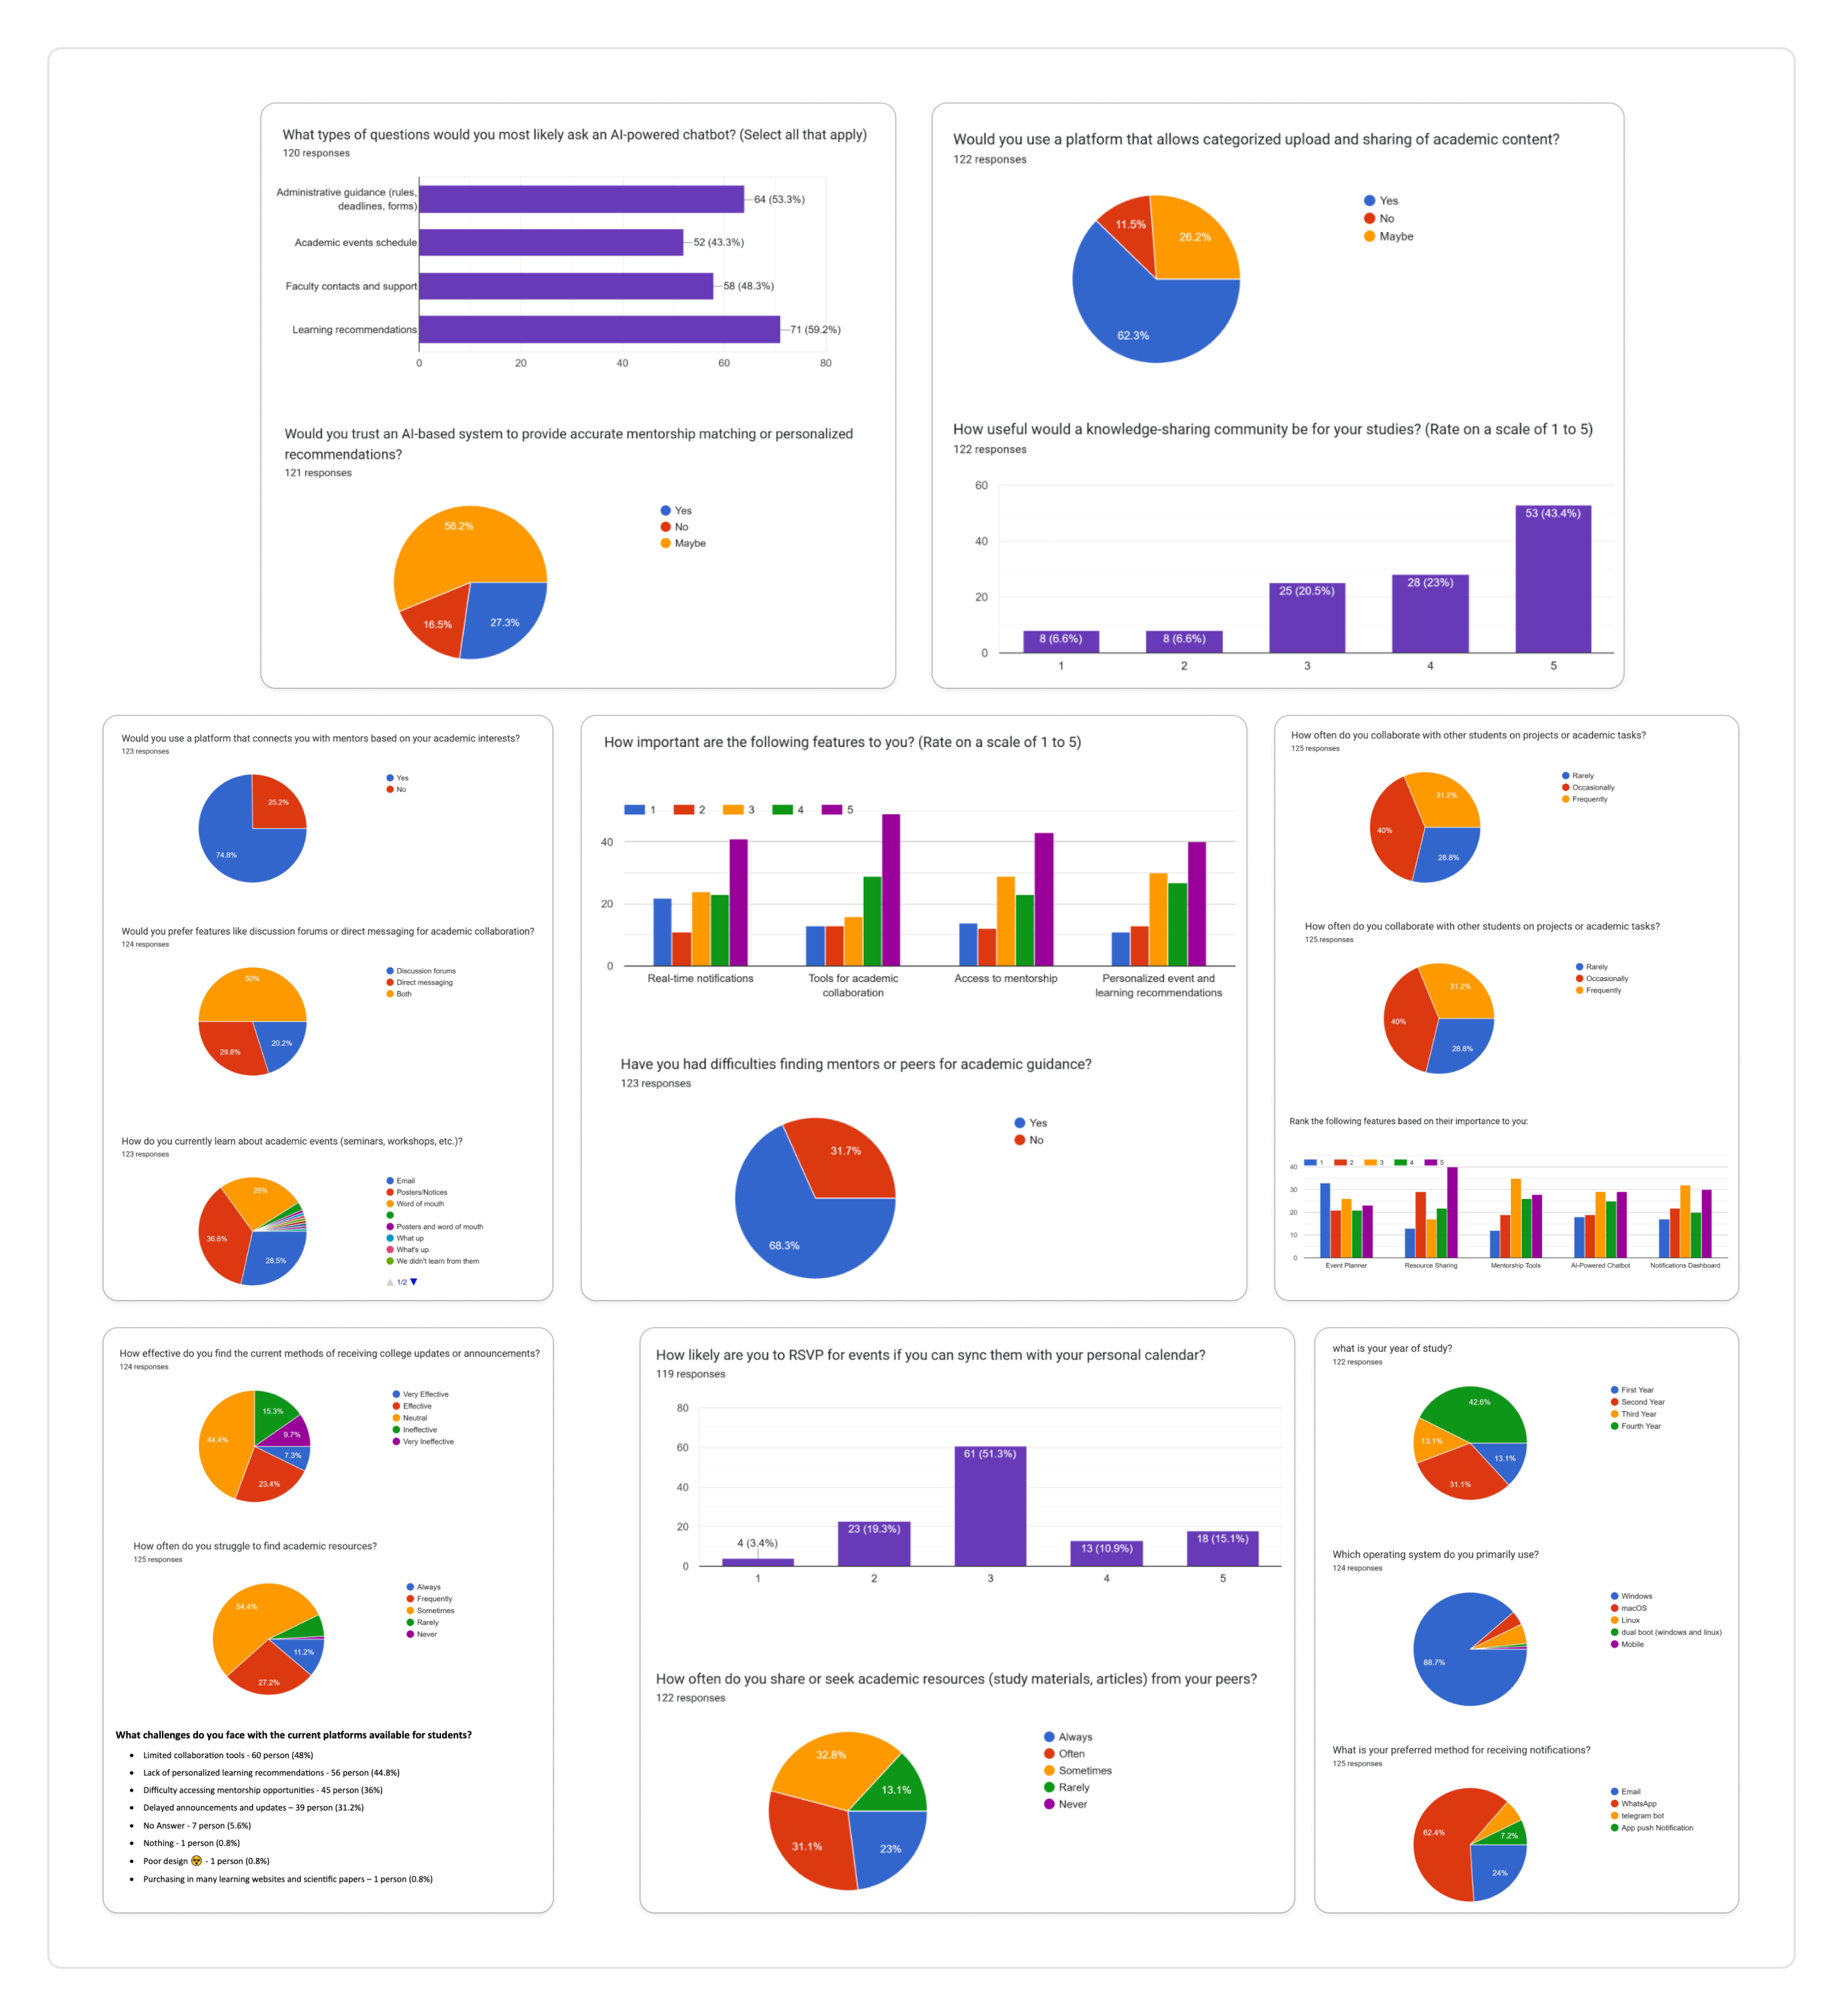
\includegraphics[width=0.8\textwidth]{images/survey_chart.png}
    \caption{Survey Results: Student Challenges with Current Academic Platforms}
    \label{fig:survey_chart}
\end{figure}

\subsection*{Key Questions in Surveys and Interviews}

The data was collected through thoughtfully structured open and closed-ended questions. Some of the most impactful questions included:

\begin{enumerate}
\item What are the biggest challenges in using current academic platforms?
\item Would you benefit from an AI chatbot for quick university-related queries?
\item How do you currently find and attend academic events?
\item Do you feel mentorship opportunities are easily accessible?
\item What additional features would improve your academic experience?
\end{enumerate}

\subsection*{User-Suggested Features and Insights}

Open-ended responses offered rich feedback and creative suggestions. A recurring theme was the demand for an intelligent, supportive, and user-friendly digital environment. Commonly suggested features included:

\begin{itemize}
\item \textbf{AI Chatbot}: To answer questions, recommend resources, send notifications, help with academic system navigation, and track learning progress weekly.
\item \textbf{Improved UX and Responsiveness}: Ease of use and accessibility were considered essential by multiple respondents.
\item \textbf{Media Player Integration}: To simplify access to video lectures and multimedia resources.
\item \textbf{OCR and PDF Analysis Tools}: For better interaction with academic documents.
\item \textbf{Study Planning and Time Management}: Tools to help students manage their workload and plan effectively.
\item \textbf{Mentorship and Peer Support}: Features to connect students with seniors, mentors, and professionals in their field.
\item \textbf{Centralized Academic Resources}: Including Google Drive-like repositories and previous-year materials.
\item \textbf{Event and Quiz Alerts}: Automated email or message notifications to keep students informed in real time.
\end{itemize}

These findings directly informed the functional and non-functional requirements of the portal, ensuring student feedback played a central role in system design.

\subsection*{Emotional Tone and Trust}

Lastly, many students expressed enthusiasm and hope that this platform would surpass current tools like Thinki, noting a desire for a ``platform that can be fully relied upon with artificial intelligence'' and praising the initiative. One respondent wrote:

\begin{quote}
``I trust you and I am looking forward to completing the rest of my university years on your wonderful platform.'' --- \textit{Moamen Sakr, Preparatory Class, Damanhour Engineering}
\end{quote}

Such testimonials underscore the responsibility and potential impact of delivering a well-engineered, student-centric platform.


\section{Functional Requirements}

These are the core features the Student Portal must support:

\begin{enumerate}
    \item \textbf{User Authentication \& Profile Management}
    \begin{itemize}
        \item Secure login with JWT authentication.
        \item Role-based access (Students, Faculty, Admins).
    \end{itemize}

    \item \textbf{AI-Powered Chatbot}
    \begin{itemize}
        \item Answer FAQs related to courses, deadlines, and campus facilities.
        \item Provide academic and administrative guidance.
    \end{itemize}

    \item \textbf{Event Management System}
    \begin{itemize}
        \item Event creation, RSVPs, and calendar synchronization.
        \item AI recommendations for relevant academic events.
    \end{itemize}

    \item \textbf{Resource Sharing \& Knowledge Base}
    \begin{itemize}
        \item Upload/download study materials and academic articles.
        \item AI-driven recommendations based on user activity.
    \end{itemize}

    \item \textbf{Mentorship Matching \& Direct Messaging}
    \begin{itemize}
        \item Match students with faculty or peer mentors.
        \item Real-time messaging and discussion groups.
    \end{itemize}

    \item \textbf{Real-Time Notifications \& Dashboard}
    \begin{itemize}
        \item Instant alerts for announcements, deadlines, and events.
        \item Customizable notifications based on user preferences.
    \end{itemize}

    \item \textbf{Collaboration Tools \& Community Forum}
    \begin{itemize}
        \item Discussion boards for academic topics and group projects.
        \item Categorized Q\&A forums for better engagement.
    \end{itemize}
\end{enumerate}

\section{Non-Functional Requirements}

These define the quality attributes of the system:

\begin{enumerate}
    \item \textbf{Performance}
    \begin{itemize}
        \item The system should handle 1,000+ concurrent users without lag.
        \item AI chatbot responses must be under 2 seconds.
    \end{itemize}

    \item \textbf{Scalability}
    \begin{itemize}
        \item Cloud-based infrastructure to support increasing student enrollment.
        \item Modular architecture for adding future features.
    \end{itemize}

    \item \textbf{Security}
    \begin{itemize}
        \item Data encryption using AES-256 and TLS 1.3.
        \item Secure API gateway with rate limiting and JWT validation.
    \end{itemize}

    \item \textbf{Usability}
    \begin{itemize}
        \item Intuitive UI/UX design for seamless experience on web and mobile.
        \item Minimal onboarding time with self-explanatory navigation.
    \end{itemize}

    \item \textbf{Reliability \& Availability}
    \begin{itemize}
        \item 99.9\% uptime with automatic failover mechanisms.
        \item Regular backups to prevent data loss.
    \end{itemize}

    \item \textbf{Maintainability}
    \begin{itemize}
        \item Codebase follows modular and well-documented practices.
        \item Version control with GitHub for continuous integration \& deployment.
    \end{itemize}
\end{enumerate}

\section{Use Case Diagram}
\begin{figure}[H]
    \centering
    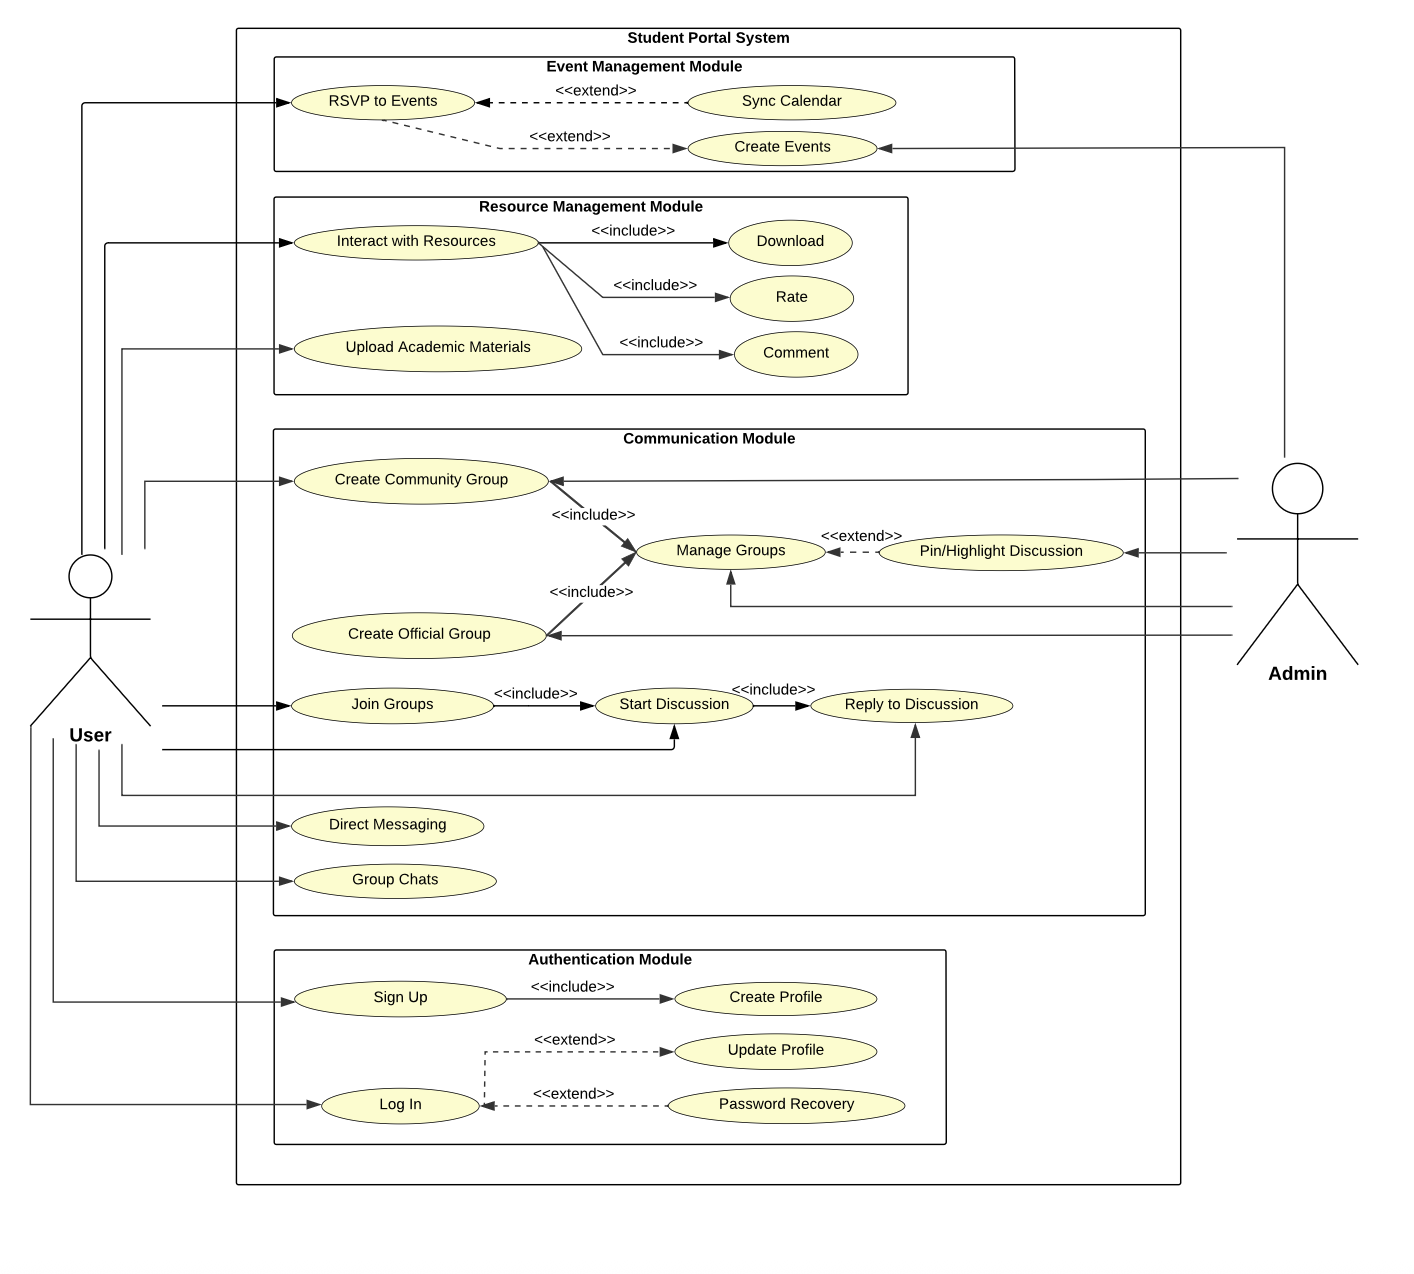
\includegraphics[width=0.8\textwidth]{images/use_case_diagram.png}
    \caption{Student Portal Use Case Diagram}
    \label{fig:use_case}
\end{figure}



\section{Use Case Tables}
\subsubsection{User Management}
\begin{table}[H]
\centering
\caption{UC-101: Sign Up}
\begin{tabular}{|l|p{10cm}|}
\hline
\textbf{Field} & \textbf{Details} \\ \hline
Actor & New User \\ \hline
Trigger & User clicks on the "Sign Up" button \\ \hline
Input & Institutional email, password, optional profile details \\ \hline
Validation Steps & 1. Verify email domain matches institutional pattern \\ 
                 & 2. Ensure password meets security criteria \\ \hline
Error Handling & 1. Display error if email is invalid \\ 
               & 2. Show password validation errors \\ 
               & 3. Alert if email is already registered \\ \hline
Output & User receives a confirmation email \\ \hline
Post-condition & Account is created and active \\ \hline
Priority & High \\ \hline
\end{tabular}
\end{table}

\begin{table}[H]
\centering
\caption{UC-102: Log In}
\begin{tabular}{|l|p{10cm}|}
\hline
\textbf{Field} & \textbf{Details} \\ \hline
Actor & Registered User \\ \hline
Trigger & User clicks "Log In" and enters credentials \\ \hline
Input & Email, password \\ \hline
Validation Steps & Match email and password to stored credentials \\ \hline
Error Handling & 1. Show "Invalid credentials" \\ 
               & 2. Account lock after multiple failed attempts \\ \hline
Output & User gains access to the dashboard \\ \hline
Post-condition & User is logged into their profile \\ \hline
Priority & High \\ \hline
\end{tabular}
\end{table}

% UC-103: Password Recovery
\begin{table}[H]
\centering
\caption{UC-103: Password Recovery}
\begin{tabular}{|l|p{10cm}|}
\hline
\textbf{Field} & \textbf{Details} \\ \hline
Actor & User who forgot their password \\ \hline
Trigger & User clicks "Forgot Password" link \\ \hline
Input & Registered email address \\ \hline
Validation Steps & 1. Verify email exists in the database \\ 
                 & 2. Ensure reset link is unique and time-limited \\ \hline
Error Handling & 1. Display "Email not found" \\ 
               & 2. Expire old reset links \\ \hline
Output & User receives email with reset link \\ \hline
Post-condition & Password is updated successfully \\ \hline
Priority & Medium \\ \hline
\end{tabular}
\end{table}

% UC-111: Create Profile
\begin{table}[H]
\centering
\caption{UC-111: Create Profile}
\begin{tabular}{|l|p{10cm}|}
\hline
\textbf{Field} & \textbf{Details} \\ \hline
Actor & New User \\ \hline
Trigger & User logs in for first time and navigates to Profile \\ \hline
Input & Profile picture, bio, academic interests, optional details \\ \hline
Validation Steps & 1. Ensure required fields are filled \\ 
                 & 2. Validate file type for profile picture \\ \hline
Error Handling & 1. Display error for invalid file types \\ 
               & 2. Allow retry with correct inputs \\ \hline
Output & Profile is saved and viewable \\ \hline
Post-condition & Profile setup is complete \\ \hline
Priority & Medium \\ \hline
\end{tabular}
\end{table}

% UC-112: Update Profile
\begin{table}[H]
\centering
\caption{UC-112: Update Profile}
\begin{tabular}{|l|p{10cm}|}
\hline
\textbf{Field} & \textbf{Details} \\ \hline
Actor & Registered User \\ \hline
Trigger & User clicks "Edit Profile" \\ \hline
Input & Updated profile details \\ \hline
Validation Steps & 1. Check file size/format \\ 
                 & 2. Validate mandatory fields \\ \hline
Error Handling & 1. Show real-time validation errors \\ 
               & 2. Allow cancel/retry \\ \hline
Output & Updates saved and reflected \\ \hline
Post-condition & Profile shows latest changes \\ \hline
Priority & Medium \\ \hline
\end{tabular}
\end{table}


\subsubsection{Communication}
\begin{table}[H]
\centering
\caption{UC-201: Direct Messaging}
\begin{tabular}{|l|p{10cm}|}
\hline
\textbf{Field} & \textbf{Details} \\ \hline
Actor & User \\ \hline
Trigger & User searches for a peer and opens a chat window \\ \hline
Input & Text message or attachment \\ \hline
Validation Steps & 1. Ensure recipient exists \\ 
                 & 2. Validate message length and attachment size \\ \hline
Error Handling & 1. Show error if recipient not found \\ 
               & 2. Notify if attachment size exceeds limits \\ \hline
Output & Message is sent and visible to recipient \\ \hline
Post-condition & Communication thread is updated \\ \hline
Priority & High \\ \hline
\end{tabular}
\end{table}

% UC-202: Group Chats
\begin{table}[H]
\centering
\caption{UC-202: Group Chats}
\begin{tabular}{|l|p{10cm}|}
\hline
\textbf{Field} & \textbf{Details} \\ \hline
Actor & User \\ \hline
Trigger & User selects/creates group chat \\ \hline
Input & Group name, description, messages \\ \hline
Validation Steps & 1. Validate group name uniqueness \\ 
                 & 2. Ensure members exist \\ \hline
Error Handling & 1. Notify name conflicts \\ 
               & 2. Alert message delivery fails \\ \hline
Output & Messages visible to group members \\ \hline
Post-condition & Group chat is active \\ \hline
Priority & Medium \\ \hline
\end{tabular}
\end{table}

% UC-211: Create Groups
\begin{table}[H]
\centering
\caption{UC-211: Create Groups}
\begin{tabular}{|l|p{10cm}|}
\hline
\textbf{Field} & \textbf{Details} \\ \hline
Actor & User, Faculty, or Admin \\ \hline
Trigger & Click "Create Group" \\ \hline
Input & Group name, description, type, optional image \\ \hline
Validation Steps & 1. Ensure name unique \\ 
                 & 2. Validate description length \\ 
                 & 3. For Official Groups: \\ 
                 & - Verify creator permissions \\ 
                 & - Validate academic purpose \\ \hline
Error Handling & 1. Show name exists error \\ 
               & 2. Notify upload failures \\ 
               & 3. Display permission errors \\ \hline
Output & Group created in appropriate directory \\ \hline
Post-condition & Official: Faculty/admin modifiable \\ 
               & Community: Creator modifiable \\ \hline
Priority & High \\ \hline
\end{tabular}
\end{table}

% UC-212: Join Groups
\begin{table}[H]
\centering
\caption{UC-212: Join Groups}
\begin{tabular}{|l|p{10cm}|}
\hline
\textbf{Field} & \textbf{Details} \\ \hline
Actor & User \\ \hline
Trigger & User clicks "Join" on group \\ \hline
Input & Selected group \\ \hline
Validation Steps & Verify group access settings: \\ 
                 & - Official: Open/Invite-only \\ 
                 & - Community: Public/private \\ \hline
Error Handling & 1. Display "Access Denied" \\ 
               & 2. Notify if at capacity \\ \hline
Output & User added as member \\ \hline
Post-condition & User receives group updates \\ \hline
Priority & Medium \\ \hline
\end{tabular}
\end{table}

% UC-213: Manage Groups
\begin{table}[H]
\centering
\caption{UC-213: Manage Groups}
\begin{tabular}{|l|p{10cm}|}
\hline
\textbf{Field} & \textbf{Details} \\ \hline
Actor & Group Owner \\ \hline
Trigger & Select "Manage Group" \\ \hline
Input & Updated details, member actions, settings \\ \hline
Validation Steps & 1. Validate permissions: \\ 
                 & - Official: Faculty/Admin \\ 
                 & - Community: Creator \\ 
                 & 2. Verify member operations \\ 
                 & 3. Check platform guidelines \\ \hline
Error Handling & 1. Show permission errors \\ 
               & 2. Display invalid operation errors \\ 
               & 3. Notify save failures \\ 
               & 4. Alert rule violations \\ \hline
Output & Group details updated \\ \hline
Post-condition & Changes reflected per guidelines \\ \hline
Priority & High \\ \hline
\end{tabular}
\end{table}

% UC-214: Start Discussion
\begin{table}[H]
\centering
\caption{UC-214: Start Discussion}
\begin{tabular}{|l|p{10cm}|}
\hline
\textbf{Field} & \textbf{Details} \\ \hline
Actor & Group Member \\ \hline
Trigger & Click "Start Discussion" \\ \hline
Input & Title, content, optional attachments \\ \hline
Validation Steps & 1. Ensure title not empty \\ 
                 & 2. Validate content length \\ 
                 & 3. Check file type/size \\ \hline
Error Handling & 1. Show invalid input errors \\ 
               & 2. Notify upload failures \\ \hline
Output & Discussion visible to members \\ \hline
Post-condition & Members can interact \\ \hline
Priority & High \\ \hline
\end{tabular}
\end{table}

% UC-215: Reply to Discussion
\begin{table}[H]
\centering
\caption{UC-215: Reply to Discussion}
\begin{tabular}{|l|p{10cm}|}
\hline
\textbf{Field} & \textbf{Details} \\ \hline
Actor & Group Member \\ \hline
Trigger & Click "Reply" on discussion \\ \hline
Input & Reply content, optional attachments \\ \hline
Validation Steps & 1. Ensure reply not empty \\ 
                 & 2. Validate attachments \\ \hline
Error Handling & 1. Show input errors \\ 
               & 2. Notify upload failures \\ \hline
Output & Reply added to thread \\ \hline
Post-condition & Members see reply \\ \hline
Priority & Medium \\ \hline
\end{tabular}
\end{table}

% UC-216: Pin/Highlight Discussion
\begin{table}[H]
\centering
\caption{UC-216: Pin/Highlight Discussion}
\begin{tabular}{|l|p{10cm}|}
\hline
\textbf{Field} & \textbf{Details} \\ \hline
Actor & Admin/Faculty/Moderator \\ \hline
Trigger & Select "Pin" or "Highlight" \\ \hline
Input & Selected discussion \\ \hline
Validation Steps & Ensure actor has permissions \\ \hline
Error Handling & Display permission errors \\ \hline
Output & Discussion pinned/highlighted \\ \hline
Post-condition & Discussion appears at top \\ \hline
Priority & Medium \\ \hline
\end{tabular}
\end{table}

\subsubsection{Resource Management}
\begin{table}[H]
\centering
\caption{UC-301: Upload Academic Materials}
\begin{tabular}{|l|p{10cm}|}
\hline
\textbf{Field} & \textbf{Details} \\ \hline
Actor & User \\ \hline
Trigger & User clicks "Upload Resource" \\ \hline
Input & File, title, description, tags \\ \hline
Validation Steps & 1. Check file type and size \\ 
                 & 2. Ensure title and description are not empty \\ \hline
Error Handling & 1. Show error for unsupported file types \\ 
               & 2. Notify if upload fails \\ \hline
Output & Resource is uploaded and visible \\ \hline
Post-condition & Others can view/download the resource \\ \hline
Priority & High \\ \hline
\end{tabular}
\end{table}

% UC-302: Interact with Resources
\begin{table}[H]
\centering
\caption{UC-302: Interact with Resources}
\begin{tabular}{|l|p{10cm}|}
\hline
\textbf{Field} & \textbf{Details} \\ \hline
Actor & User \\ \hline
Trigger & Select resource to interact \\ \hline
Input & Comment, rating, or download \\ \hline
Validation Steps & 1. Validate rating scale \\ 
                 & 2. Ensure comments not empty \\ \hline
Error Handling & Notify if save fails \\ \hline
Output & Interaction recorded \\ \hline
Post-condition & Enhances engagement \\ \hline
Priority & Medium \\ \hline
\end{tabular}
\end{table}


\subsubsection{Event Management}
\begin{table}[H]
\centering
\caption{UC-401: Create Events}
\begin{tabular}{|l|p{10cm}|}
\hline
\textbf{Field} & \textbf{Details} \\ \hline
Actor & Faculty, Admin \\ \hline
Trigger & Faculty/Admin clicks "Create Event" \\ \hline
Input & Event name, date, time, location, description \\ \hline
Validation Steps & 1. Check date and time validity \\ 
                 & 2. Ensure required fields are filled \\ \hline
Error Handling & 1. Show error if date/time is invalid \\ 
               & 2. Notify if image upload fails \\ \hline
Output & Event is created and visible \\ \hline
Post-condition & Users can view and RSVP \\ \hline
Priority & High \\ \hline
\end{tabular}
\end{table}

% UC-402: RSVP to Events
\begin{table}[H]
\centering
\caption{UC-402: RSVP to Events}
\begin{tabular}{|l|p{10cm}|}
\hline
\textbf{Field} & \textbf{Details} \\ \hline
Actor & User \\ \hline
Trigger & Click "RSVP" on event \\ \hline
Input & Event selection \\ \hline
Validation Steps & Ensure event not full \\ \hline
Error Handling & Notify if full or fails \\ \hline
Output & RSVP recorded \\ \hline
Post-condition & User receives updates \\ \hline
Priority & Medium \\ \hline
\end{tabular}
\end{table}

% UC-403: Sync Events to Calendar
\begin{table}[H]
\centering
\caption{UC-403: Sync Events to Calendar}
\begin{tabular}{|l|p{10cm}|}
\hline
\textbf{Field} & \textbf{Details} \\ \hline
Actor & User \\ \hline
Trigger & Click "Sync to Calendar" \\ \hline
Input & Calendar integration \\ \hline
Validation Steps & Ensure permissions granted \\ \hline
Error Handling & Notify sync failures \\ \hline
Output & Event added to calendar \\ \hline
Post-condition & Event in personal calendar \\ \hline
Priority & Low \\ \hline
\end{tabular}
\end{table}